\begin{figure}[tbp]
    \centering
    % both panels share one height so their tops and bottoms line up
    \newlength{\frontierheight}\setlength{\frontierheight}{0.322\textwidth}% set outside the subfigures, where \textwidth is the page width
    \begin{subfigure}[b]{0.47\textwidth}
        \centering
        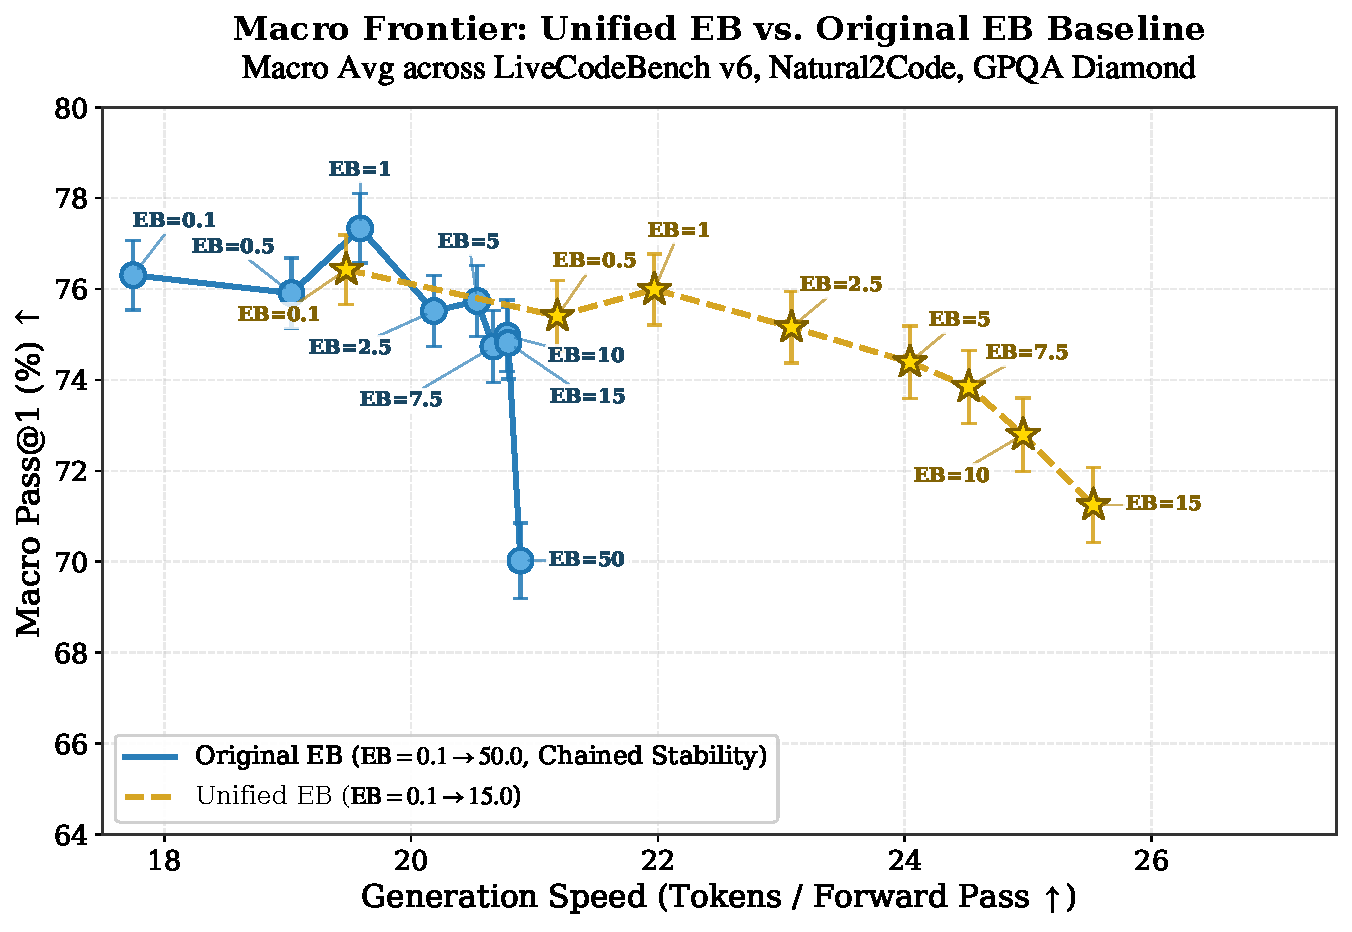
\includegraphics[height=\frontierheight]{images/fig_macro_frontier_original_vs_unified.pdf}
        \caption{Original vs.\ unified stopping.}
        \label{fig:unified-vs-orig}
    \end{subfigure}
    \hfill
    \begin{subfigure}[b]{0.51\textwidth}
        \centering
        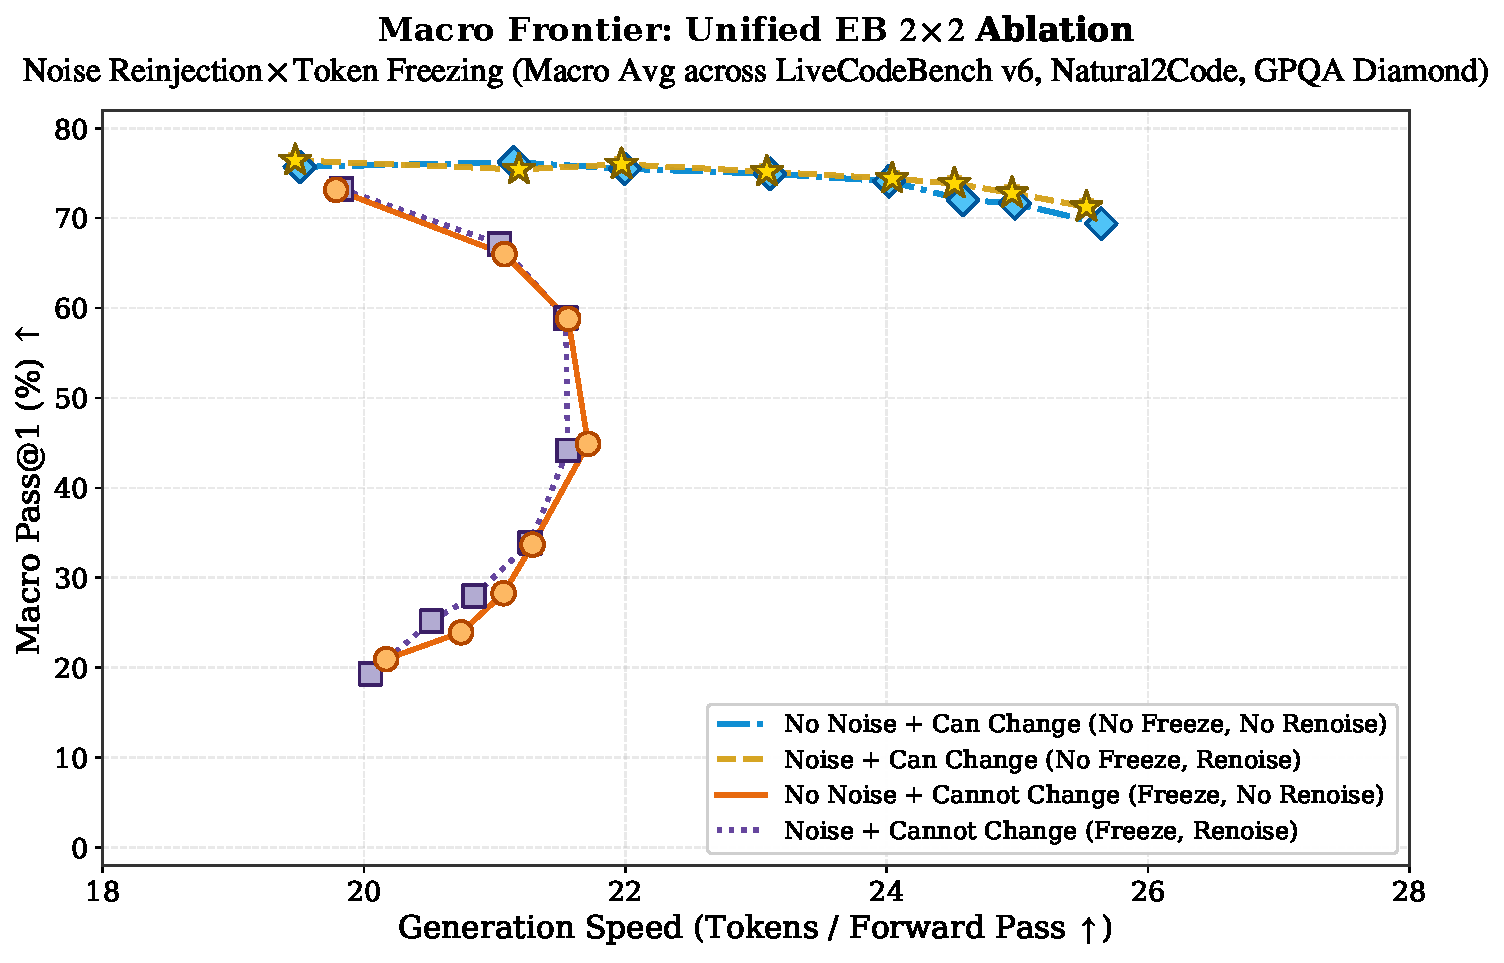
\includegraphics[height=\frontierheight]{images/fig_macro_frontier_unified_ablation_2x2.pdf}
        \caption{Frozen vs.\ base EB sampler.}
        \label{fig:frozen-eb-frontier}
    \end{subfigure}
    \caption{\textbf{(a)} The unified stopping criterion matches the original at a slight speedup. \textbf{(b)} Pareto frontier of the modified EB sampler: larger entropy bounds trade performance for throughput, and the frozen variant degrades much faster than the base version, showing that the flexibility of the uniform diffusion process drives the frontier.}
    \label{fig:eb-frontiers}
\end{figure}
